This chapter gives an introduction to literature from the museum field, starting with the ongoing transitional shift to a \emph{new} museology. The chapter will then introduce concepts and terms from exhibition and dissemination practise to create a vocabulary for talking about museum subjects and roles in this thesis. Then we will progress into sustainability as a topic representative of a contemporary discourse being addressed in a museum. The chapter is then rounded off with literature on the application and use of technology and interactive installations in "modern museums."


\section{The new museology}
In 1989, Peter Vergo coined the term \emph{the new museology} in a book bearing the same name. Museology is the study of museums, their history and underlying philosophy, and the various ways in which they have during the passing of time, been established and developed \autocite[p.1]{vergo_museology_1989}. Vergo argues that beyond the physical material like handouts or information panels, there is a subtext comprising diverse and often contradictory strands woven from the intellectual, political, or educational preconceptions of the museum stakeholders, e.g. the museum director, the curator, the scholar or the designer \autocite[p.3]{vergo_museology_1989}. Rather than old considerations like administrative tasks, conservation techniques, financial well-being, or, success or neglect in the eyes of the public, the subject matter that should be more questioned or discussed should be more concerned with the museums \emph{purpose} rather than museum \emph{methods} \autocite[p.3]{vergo_museology_1989}. Vergo would therefore define the \emph{new} museology simply as a state of widespread dissatisfaction with the \emph{old} museology considerations. "Unless a radical re-examination of the role of museums within society takes place", Vergo declares that museums in this country (referring to the UK), and possibly elsewhere, may likewise find themselves dubbed 'living fossils' \autocite[p.4]{vergo_museology_1989}.

Throughout this thesis project, it has become quite evident that Norwegian museums are making efforts to renew themselves and embrace the possibilities that interactive exhibition curatorship could encompass. Moreover, that interactive and audiovisual elements are almost self-evident parts of the exhibition strategies in Norwegian museums \autocite[p. 59]{melding23}. Compared with other countries' museums, e.g., the Louvre in Paris, France, which could be an example of Vergo's traditional museum or old museology tradition, where the art represents or at least is very tightly coupled with the french cultural heritage and national identity. This means conservative voices in public can stand in the way of renewal or change, making the transformative strategies more elongated. However, literature agrees that the museum world has undergone radical changes since the 1970s- and 80s. \emph{"Political and economic pressures have forced its professionals to shift their attention from their collections toward visitors. Whereas in the past, the museum tended to be exclusive and elitist, signs of a progressive opening-up and greater accessibility have appeared. A climate of increasing reflexivity within the profession is identified as a 'new museology'."} \autocite[p. 84]{ross_interpreting_2015}.


\subsubsection{Museum experience design}
Recent literature in the HCI field concerned with museums agrees that the museum world is rapidly changing from being collection-centered to being community-centered and for the public \autocite[p. 1]{vermeeren_museum_2018}. And that museums have become a place for education and learning, dialogue and debate \autocite{hein_1998}, \autocite{hooper_1994}, \autocite{Roberts_1997}. New ways of involving the public more meaningfully have emerged, but there is still much to uncover; experiences in museums have become more engaging by extending the experience beyond the physical visit. \autocite{vermeeren_museum_2018} presents four key themes relevant for designers concerned with experience design in museums:

\begin{itemize}
    \item Engaging the public,
    \item Cultivating diverse audiences,
    \item Availing ourselves of the benefits of digital technology,
    \item and, Leveraging museums’ roles as players in larger economic and cultural ecosystems.
\end{itemize}

This thesis and its research inquiries positions itself in the first key theme presented; engaging the public, with the goal to understand more about how one can design meaningful interactive experiences in a museum space. \emph{Too often we (the museum) prioritize our mandate to hold and protect our collections and stop short of making them relevant to today’s audiences, real or potential. Too often we are zoomed way too far in on our objects, and lose sight of what people less invested might know, think, or want from us.}\autocite[p. 1]{vermeeren_museum_2018} In light of this, \autocite{vermeeren_vincent_2018}'s case on \emph{Becoming Vincent} is instructive where it among the findings is implied how "the importance of and attention to content is related to the increasing value associated with craftsmanship, in the belief that this will provide a real, genuine, and authentic experience" \autocite[p. 298]{vermeeren_vincent_2018}. "When we pull our focus back from the individual museum and its obsession with its objects, we find a larger community outside that is largely indifferent to our obsessions, and needs a story, even a superstar, to motivate their interest" \autocite[p. 1]{vermeeren_museum_2018}. "This is why storytelling can help turn any experience into a memorable and meaningful experience, by unlocking values that would otherwise be not so immediately recognizable by the listeners" \autocite[p. 299]{vermeeren_vincent_2018}. Then, "a struggle emerges between the museum’s role as protector of authentic objects and the “facts” around them and its role as a site of experiences—preferably extraordinary ones, because if not, why bother? "\autocite[p. 1]{vermeeren_museum_2018}. \emph{"So, while digital apps take us on mobile adventures and open up trails of wonder for some, the vast majority of our visitors still default to analog first and foremost. The more we can design for blended environments that mix the virtues of analog and digital affordances in mutually reinforcing ways to foster a context for meaningful engagement with museum objects, the better off we’ll be"} \autocite[p. 1]{vermeeren_museum_2018}. This show how the HCI community is increasingly interested in, and can benefit from, understanding more about how technology-use impacts the human experience of meaning and foster meaningful user experiences in museum contexts.

\section{Exhibition and dissemination practise}
In this section, I will present terms and concepts to explain what I mean when I talk about exhibition and dissemination practice. This lays the foundation for the vocabulary which I have adopted throughout the literature review and formatively guided data gathering and research inquiries. As supported by the Oxford dictionary of English definitions of \emph{exhibition} and \emph{dissemination} in Figure 2.1, the way exhibition and dissemination practice is understood and used in this thesis is as follows: dissemination as in the act and action of spreading information in the context of an exhibition displaying works of art, items of interest, and interactive installations in a museum.

\begin{figure}[H]
\centering
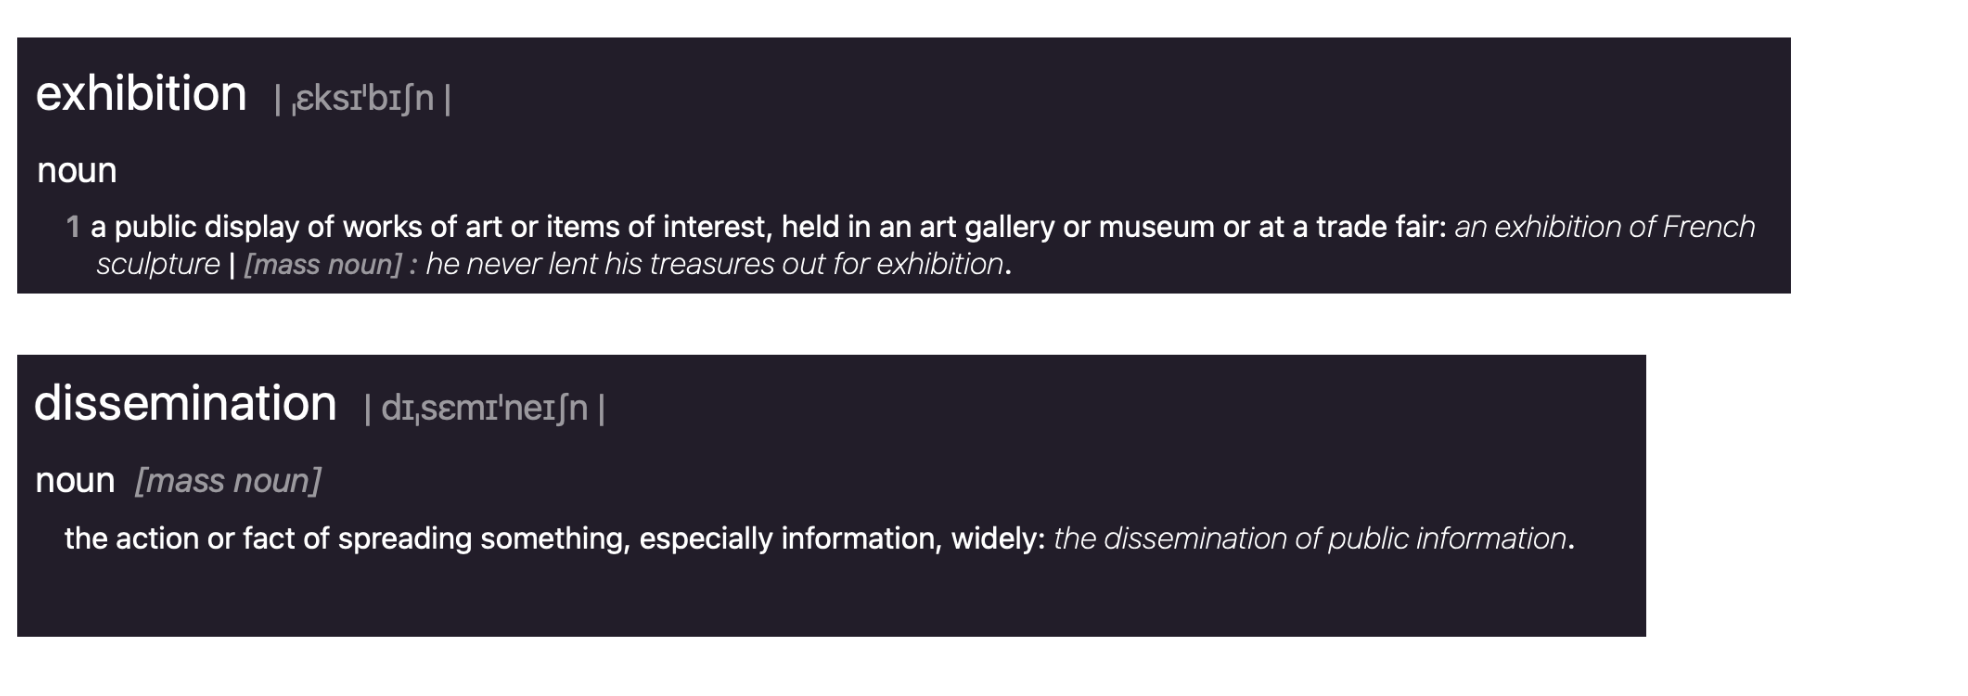
\includegraphics[width=14cm]{pictures/background/exh_diss.png}
\caption{Exhibition and dissemination practice}{\autocite{Oxford_dictionary}}
\end{figure}


\subsection{Understanding the museum discourse}
Coming into this thesis project, I knew very little about how a museum worked or functioned. Wanting to learn more about how narrative play a part in telling a story and conveying a message, I came across \autocite{Miekebal_book}'s writings on cultural analysis and discourses in the museum. Coming from a humanities background, she proposes a perspective on what differentiates the “new” from the “old” museology. According to her, the museum is seen as a discourse and the exhibition as an utterance within that discourse. She calls this a discursive perspective. By bringing this discursive perspective to the museum, it has the possibility to "deprive the museal practice of its innocence, and provide it with the accountability it and its users are entitled to" \autocite[p. 214]{Thi_book}. Part of her argument and critique is that politics come straight out of, or more precisely are bound up with, the museal discourse \autocite[p. 214]{Thi_book}. To deal with this, she suggests a threefold direction for museology researchers. First, she suggests systematically analyzing the narrative-rhetorical structure of the specific museum to refine the categories and deepen insight into their effects. Secondly, she suggests looking at the connection between the museal discourse and the institutions' foundation and history. Thirdly, she sees the need to do a self-critical analysis of the museal discourse as a consequence of the nature of discourse. \autocite{Miekebal_book} argue that in the study of museums, one should look at the museum and question:

\begin{itemize}
    \item What museum fiction do the museum tell? 
    \item Who is speaking the museum fiction?
    \item Who is the expository agents?
    \item And what is the museums expository agency?
    \item What is spoken? 
    \item Is the museum telling, showing or showing off?
\end{itemize}

These concerns make up the foundation for seeing the museum for what it is and what it presents up against what it represents. According to \autocite{Miekebal_book}, the museum itself is the expository agent. Putting forward the expository agent that “speaks” the text in the verbal panels transforms the one with a commentary on the other. Making it possible to judge whether the fiction of the museum's expository agency aligns with the expository agent's vision or not. Different museums speak different fictions, e.g., art, science, or, cultural heritage. What these fictions have in common is that they show their objects, not their own hand or voice \autocite{Miekebal_book}. The way she sees it, showing, if it refrains from telling its own story, becomes showing off. The displays can then point at their discourse as a sign system put forward by a subject, and one can look for issues of cultural moralism or cultural imperialism. Her studies are concerned with and derived from the context of looking at ethnographic museums that display ethnic objects and artefacts representing cultures and cultural properties from the past. She raises the question if former colonists are entitled to hold onto objects taken by their ancestors from former colonies, or should they give these back to the country of origin to the ancestors whose inhabitants were their original owners? This is a debate totally out of scope for this thesis but relevant in understanding the implications a discourse can have. The way I see it, sustainability and the climate crisis is a complex discourse that shares some of the same dynamics that the colonist- discourse does in terms of the uneven distribution of the cause-effects of climate change — potentially resulting in cultural moralism. As we can see from the Oxford dictionary of English in Figure 2.2, the way \emph{discourse} is understood and used in this thesis is to reference a topic or theme in the museum context, talking about either the exhibition discourse or the museum discourse.

\begin{figure}[H]
\centering
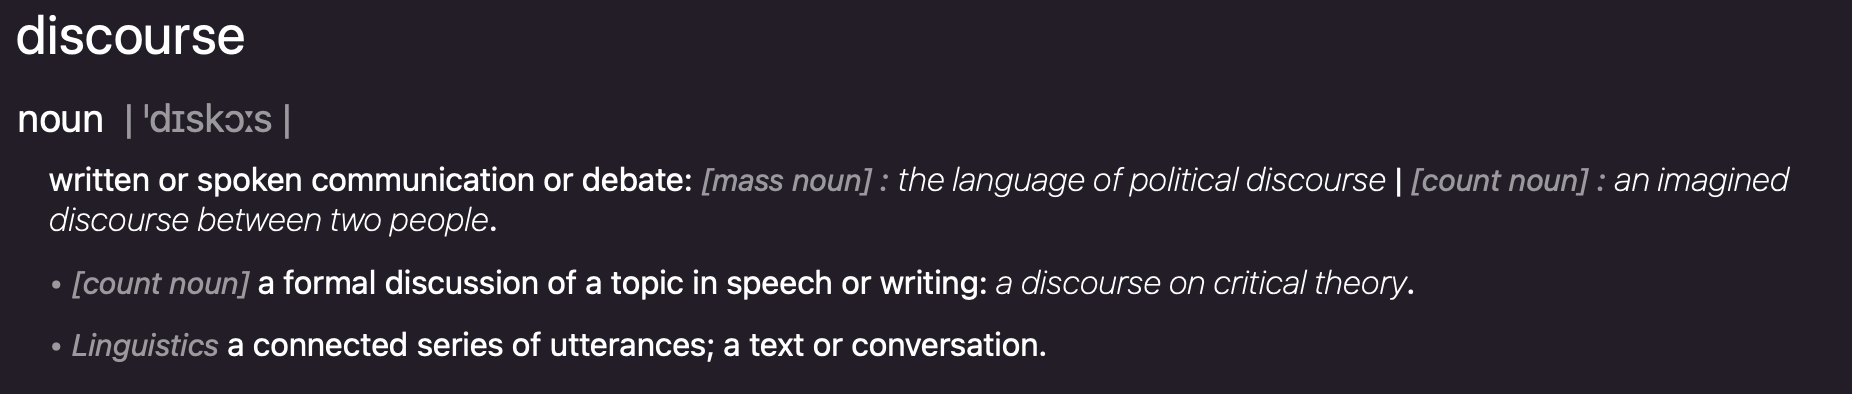
\includegraphics[width=12cm]{pictures/background/discourse.png}
\caption{Museum discourse}{\autocite{Oxford_dictionary}}
\end{figure}
 
I think this critical discourse-oriented perspective is necessary in a museum context or exhibition space addressing sustainability because the intention of making a meaningful interactive experience is also about strengthening the message conveyed by the museum. Both the designer and especially the museum's expository agents need to be aware of and able to answer the moral and ethical questions raised regarding what the message they convey, actually conveys. And that the act of strengthening that message through interactivity sends people out of the museum with reflections and thoughts that hopefully leads to social action like climate action or higher climate consciousness. There has been increasing interest in the HCI community in considering how technology-use impacts the human experience of meaning \autocite{light_design_2017}, questioning what a good design for an existential crisis is. "In the Anthropocene age, shocks of all kinds are raising questions about the future and value of humankind." \autocite[p. 723]{light_design_2017}. Light et al. argues that while there are increasing indifferences to the ecological consequences of the world, ultimately there is a growing sense that, without fast action at every level of society, we cannot outrun crisis \autocite[p. 723]{light_design_2017}. "Institutional humiliation comes in many digital guises", and Light et al. highlight the problem of techno-paternalism that nudges users toward behavior identified by others as positive, right or useful - an intensification of system efficiency at the expense of flexibility and the absence of empathetic hearing \autocite[p. 727]{light_design_2017}. Can this be an example of a modern-day concern for cultural moralism in museum exhibition and dissemination practice? 
Technologists and designers are implicated in this wave of change and uncertainty because the implications of the work they do, claims a stake in the production of futures \autocite[p. 723]{light_design_2017}. "As makers, we are practical people, as well as dreamers and theorists, and if there is no more “business as usual”, we can choose to have a role in producing alternative narratives for present generations of humans and those who depend on them, such as other species and unborn children." \autocite[p. 723]{light_design_2017}.


\subsection{Artefacts, artworks, and interactive installations}
As we have learned, the artefact and the artwork is central pieces for disseminating the museums discourse. In this section we will see how the two differ in terms of what they represent, and question the role of the interactive installation in the museum. 

\emph{The very act of collecting has a political, ideological, or aesthetic dimension that cannot be overlooked} \autocite[p. 2]{vergo_museology_1989}. Vergo questions, "what makes certain objects, rather than others 'worth' preserving? Answering his own question, he explain that "the original intention behind the establishment of museums was that they should remove artefacts from their current context of ownership and use, and insert them into a new environment which would provide them with a different meaning" \autocite[p. 6]{vergo_museology_1989}. "The essential feature of museums - and what differentiates them from the many extensive private collections which preceded them - was, at first, that the meanings which were attributed to the artefacts were held to be arbitrary; and, second, that the collections should be accessible to at least a portion of the public, who where expected to obtain some form of educational benefit from the experience" \autocite[p. 6]{vergo_museology_1989}. "A museum is an attractive object of study because it requires interdisciplinary analysis; it has the debate on aesthetics at its core, and it is essentially a social institution" \autocite[p. 202]{Thi_book}. The heritage museum conserves and exhibits artefacts, while the art museum, works of art. It seems obvious what differs between the artefact vs. the artwork, yet they differ in what they represent. Both the artefact and the artwork is charged with cultural meaning. It tells us about a more extensive cultural situation, e.g., aesthetic conceptions or world views, conceptions of representations, or the social relevance of art \autocite[p. 206]{Thi_book}. However, these meanings are only yielded if we can “read” them or is put in some context that illuminates the cultural meaning \autocite[p. 206]{Thi_book}.

The term artefact suggests a man made object charged with cultural meaning which can, if studied carefully, offer us information on the society in which it has been created \autocite[p. 205]{Thi_book}. The difference between the artefact according to the above definition and the common idea of art is that the former takes for granted what the other represses: the possibility of cultural difference \autocite[p. 205]{Thi_book}. Instead, artworks are viewed as standing for an aesthetic, and is therefore considered metaphors, transferring their specific aesthetic to the one current sufficient to make the work “readable” as art, regardless of what it could tell us about the culture it comes from \autocite[p. 206]{Thi_book}. While the ethnic artefact, in contrast, is first and foremost considered to be a representative of the larger context of the culture it comes from \autocite[p. 206]{Thi_book}, hence, it is not a metaphor but a synecdoche. Synecdoche is the figure of rhetoric where an element, a small part, stands for the whole simply by virtue of its being a part of that whole \autocite[p. 206]{Thi_book}. Thus the artefact is only readable as culture, no matter what aesthetic qualities it may also have.

Then comes the question, what does the interactive artefact or installation represent? As far as my literature search goes, there is not so much attention given to the role of the interactive artefact or installation in the HCI community. The community seems to be more interested in what makes the installation engaging and how it can provide an engaging experience for the visitor and groups, as evident in the works of \autocite{hornecker_learning_2006}, and \autocite{ciolfi_designing_2012}. As evident in the Oxford dictionary of English in Figure 2.3, the way the interactive installation is understood and used in this thesis is how the \emph{installation} refers to an artefact piece of technologically enhanced equipment, constructed within and \emph{for} a specific exhibit or discourse. And that the \emph{interactive} aspects refer to the installation allowing a two-way flow between a computer and the computer-user, where the installation responds to a visitor's input through a tangible interface.

\begin{figure}[H]
\centering
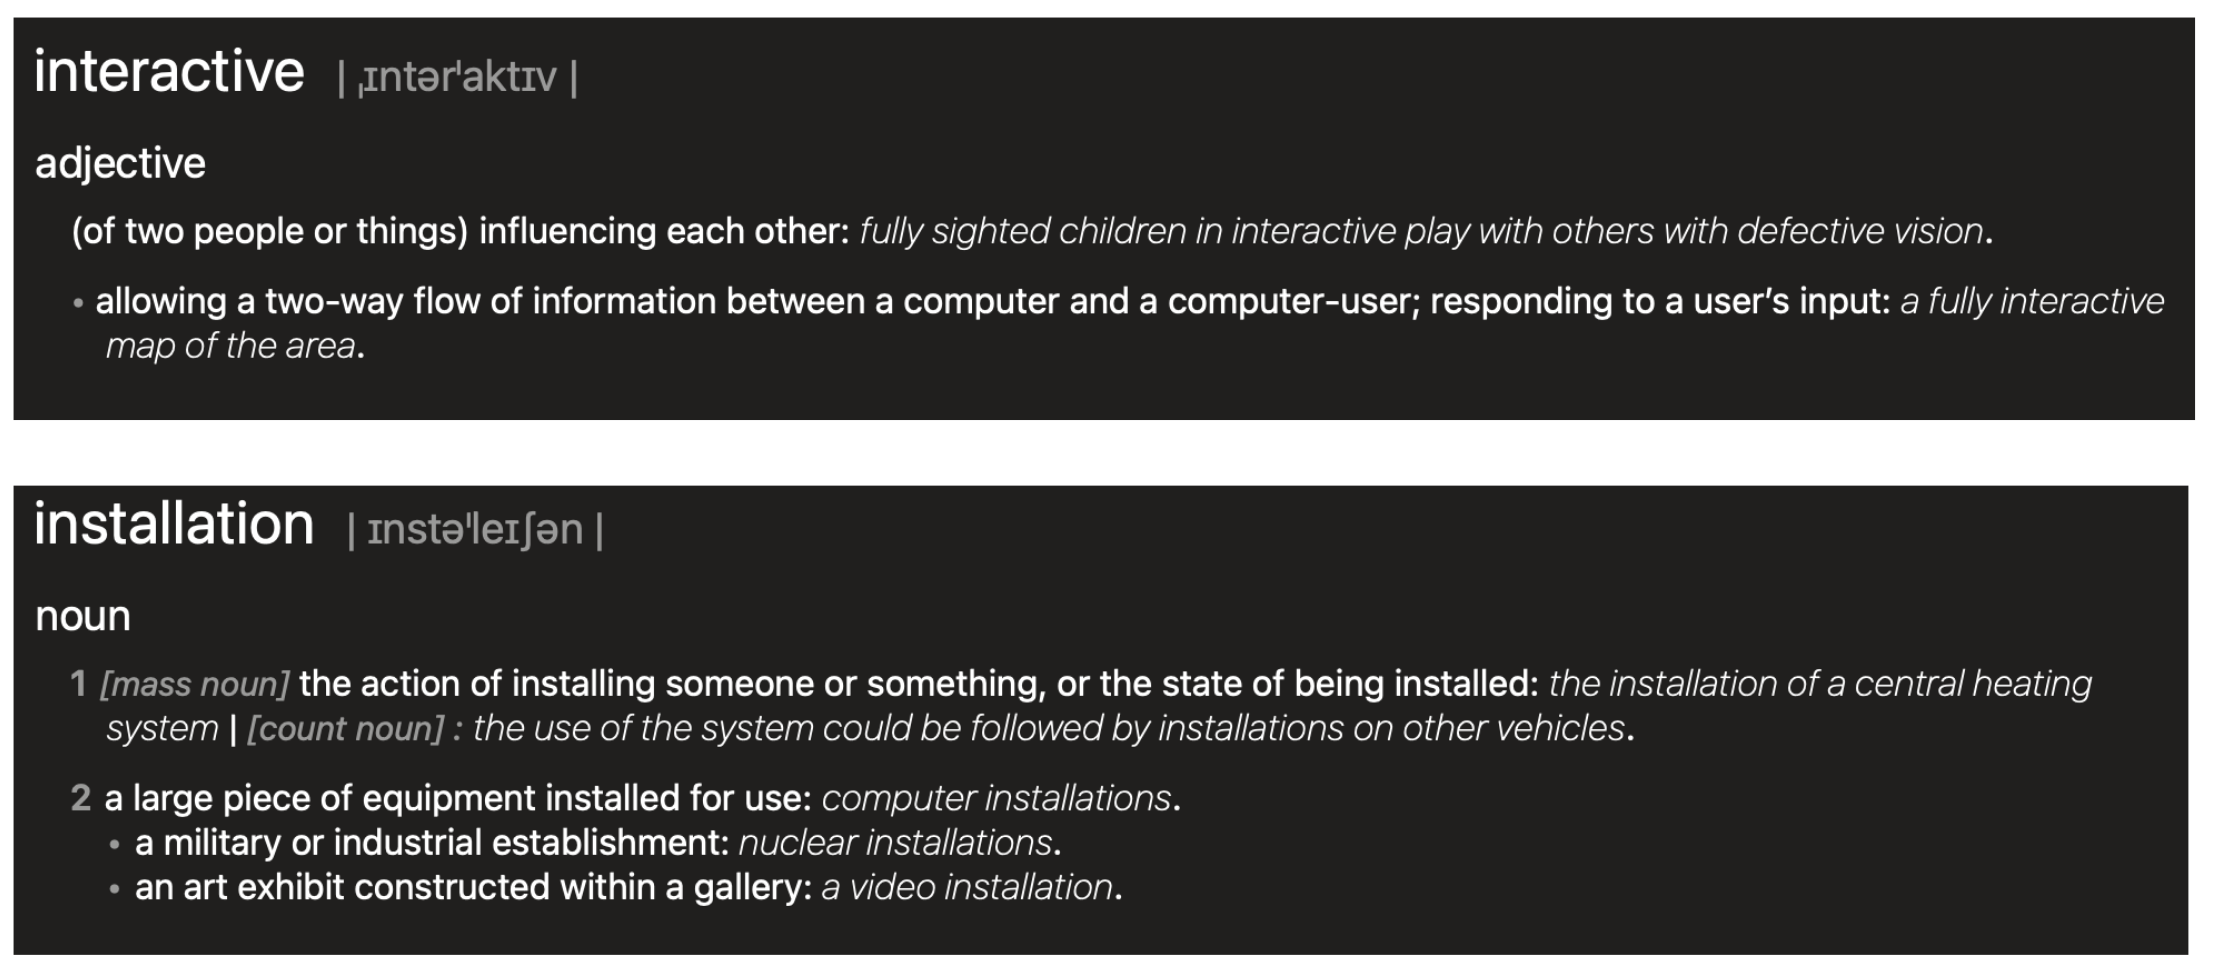
\includegraphics[width=12.5cm]{pictures/background/interactive_installation.png}
\caption{Interactive installation}{\autocite{Oxford_dictionary}}
\end{figure}


\subsection{The curatorial function}
Then comes the question of what role the designer have in the museum space, introducing, supporting or extending the museum discourse and exhibition practise? In this section I present museum literature on the curatorial function, as a means to understand the traditional museum-designer.

The curator are, above all, the institutionally recognised experts of the art-world establishment, whether they operate inside an institution or independently \autocite[p. 22]{Thi_book}. More than art-critics or gallery dealers, they establish the meaning and status of contemporary art through its acquisition, exhibition, and interpretation \autocite[p. 22]{Thi_book}. To a greater extent than other art-world professionals, curators additionally depend on an established infrastructure to support their efforts. "This infrastructure includes institutionalised networks, such as those provided by museums, galleries, or alternative spaces; financial sponsors, whether public, private or corporate, and teams of technical or professional experts" \autocite[p. 22]{Thi_book}. Curators are the sanctioned intermediaries of these institutional and professional networks on the one hand, and; artists and audiences on the other. The curatorial function is, thus, inherently restricted by the interests of the larger or more powerful groups and constituencies in the museum \autocite[p. 22]{Thi_book}. "By selecting, framing and interpreting peripheral art in exhibitions and exhibition catalogues, for instance, art curators can claim to be shaping a more democratic space where specific cultural groups can recognise themselves" \autocite[p. 23]{Thi_book}. "As the debates of recent years have shown, “identity” is not an “essence” that can be translated into a particular set of conceptual or visual traits" \autocite{Miekebal_book}, it is, rather a negotiated construct that results from the multiple positions of the subject vis-a-vis the social, cultural and political conditions which contains it \autocite[p. 23]{Thi_book}. "How then, can exhibitions or collections attempt to represent the social, cultural and political complexities of groups without reducing their subjects to essentialist stereotypes?" \autocite[p. 23]{Thi_book}.

"This situation places the cultural broker at the very core of a contradiction: on one hand, she can be credited for helping to tear down artworld hierarchies, seemingly democratizing the space for cultural action; on the other hand, in a market scenario where “identity” can only be a reductive construct, the framing and packaging of images of the collective self can only result in a highly delusionary enterprise" \autocite[p. 23-24]{Thi_book}. The tensions of this contradiction confront art curators with a dilemma; where should they position themselves vis-a-vis the identities of the groups they claim to respect? \autocite[p. 24]{Thi_book}.

Designers and traditional museum curators have a lot in common. As we have read, they have many similar considerations in synthesizing and designing an exhibition against a discourse, connecting the exhibition agency to the visitor's journey. In this thesis, the \emph{curatorial function} is seen and used as one of the considerations the designer involved in designing a whole, or part of, a museum experience. Following the Oxford dictionary of English in Figure 2.4, the curatorial function relates to the selection and organization of a museum or other collection as part of the designer's responsibility. In light of our earlier readings on the museum discourse, cultural moralism, and the role of the interactive installations, the designer's responsibility should encompass a deliberate consideration of these perspectives when introducing interactivity to the exhibition journey.

\begin{figure}[H]
\centering
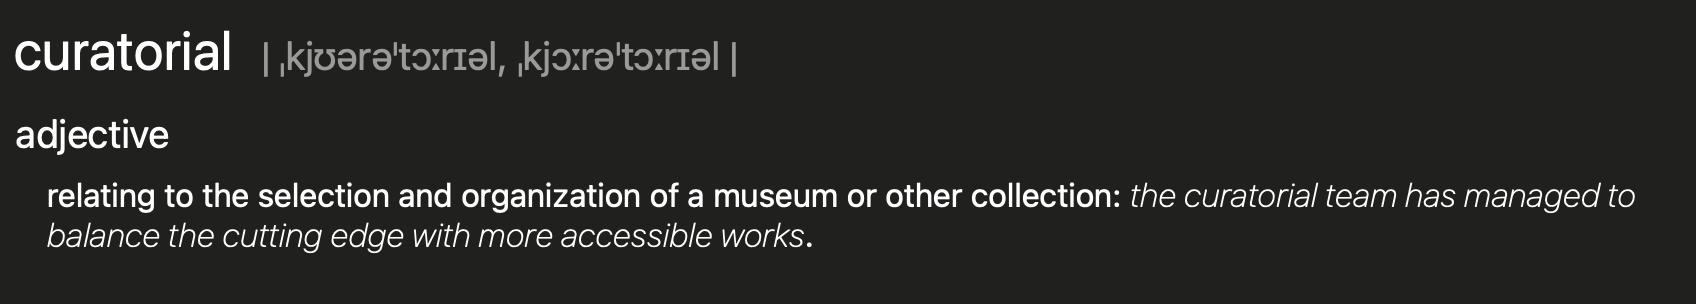
\includegraphics[width=12.5cm]{pictures/background/curatorial.png}
\caption{The curatorial function}{\autocite{Oxford_dictionary}}
\end{figure}

\subsection{The narrative of walking through a museum}
To help look at what happens in a museum, Bal is guided by the notion that the gesture of showing can be considered a discursive act. According to her, exhibiting a subject through putting “things” on display creates a subject/object dichotomy \autocite[p. 3]{Miekebal_book}. The dichotomy is a division or contrast between two things that are represented as being opposed or entirely different. The dichotomy enables the subject to make a statement about the object, while the object is there to prove evidence or the statement's truth. The addressee for the statement is the visitor, viewer, or reader \autocite[p. 3]{Miekebal_book}. The discourse surrounding the exposition, or, more precisely, the exposition's discourse, is “constative”: informative and affirmative (Bal, p. 3). The very fact of exposing the object —presenting it while informing about it — impels the subject to connect the “present” of the object to the “past” of their making, functioning, and meaning \autocite[p. 4]{Miekebal_book}. This is one of the levels giving the exposition a narrative quality. The other level where narrative can occur is the necessarily sequential nature of the visit, the “walking tour” \autocite[p. 4]{Miekebal_book}. The “walking tour” is explained to bind the elements of the exposition for the viewer together, where the narrative of walking through a museum is comparable to the narrative of reading a book.

The reason for Bal’s attention to museums is the actual, concrete “literal” exhibition of things in museums and galleries. She proposes that the tools to conduct cultural analysis in museums are best selected and employed to integrate rhetoric and narratology. Rhetoric helps to “read” not just the artefacts in a museum but also the museum and its exhibitions themselves \autocite[p. 7]{Miekebal_book}. At the same time, the narratological perspective provides meaning to the otherwise loose elements of such a reading \autocite[p. 7]{Miekebal_book}. Most importantly, the analysis aims to yield, on the one hand, an integrated account of the discursive strategies put into effect by the museum's expository agent (the curators), and, on the other hand, the practical process of meaning-making these strategies suggest to the visitor \autocite[p. 7]{Miekebal_book}. The reading itself, then, becomes part of the meaning it yields.

For my study of how one can design meaningful, interactive experiences in a museum space that addresses sustainability, this perspective is relevant because it enables me to look into the sustainability domain with the help of vocabulary derived from museology and cultural analysis. In similar museums, like heritage museums displaying ethnic types of discourses - cultural analysis has helped identify cultural moralism and imperialism in museums. I hypothesize that cultural analysis in museums addressing sustainability issues could reveal power structures or tensions in the museum's dissemination and exhibitory practice. Or perhaps moralism? Bal accounts for the museum itself being an expository agent and having an expository agency. The exposition, both in the broader, general sense of “exposing an idea” and in the specific sense of being an exhibition pointing at objects. By dissecting and putting forward the expository agent who is implicitly “speaking” throughout the exhibition design about the objects on display, one can see how one comments on the other. Bal also explains how different museums speak different “fictions,” as they call it, where, e.g., the MUNCH museum displays art and is namely an art museum. On the other hand, Klimahuset displays the science of climate history and change, and Bal would classify Klimahuset as an ethnographic museum. The distinction between the ethnographic museum and the art museums can help us understand the importance of addressing this central discursivity and of interpreting its effects. However, in this thesis, we are not so much interested in these classifications. We are simply noting how the genre to which a museum allegedly belongs is in itself part of the frame that puts pressure on the meanings it will produce.


\subsection{Dialogical engagement}
As accounted for in the latter sections, \autocite{vergo_museology_1989}, \autocite{Thi_book}, \autocite{Miekebal_book}, and \autocite{light_design_2017}, we have read how museums started off as institutions focusing on collecting and preserving objects, open for the public to come and watch. Furthermore, the primary purpose of visitors coming to the museum was to see the original objects. Moreover, this tradition has changed, especially in the last few years, and museums are starting to embrace a more visitor-focused approach to curating new exhibitions to engage a broader audience. Furthermore, visitors are demanding more engaging experiences at the museum. Vermeeren et al. indicate how "museums have so much to learn from Human-Computer Interaction (HCI), and the enormous scientific literature that has developed around User experience (UX)" \autocite{vermeeren_museum_2018}.\emph{"A first notable shift saw the museums move from a collection focus to a visitor focus and from a mission for objects preservation and access provision to a mission of offering meaningful engagements with the collection and rewarding learning experiences for their public"} \autocite[p. 3]{vermeeren_museum_2018}. \emph{The concept of ‘museum experience’ is the pinnacle of this historical shift, as it implies a focus on the visitor and connections between visitors and objects rather than a focus on collections. Over time, new types of museum experiences gradually emerged} \autocite[p. 3]{vermeeren_museum_2018}. "The degree of sophistication and immersion increased exponentially when experiences started to be enhanced by the integration of interactive and digital media" \autocite[p. 3]{vermeeren_museum_2018}. "In many science and technology museums, for example, visitor engagement and participation are uplifted through the use of new media (e.g., video games, interactive installations, and other forms of edutainment) to encourage visitors to engage with the content on exhibit, to experiment with the techniques on display and to appropriate the visiting experience by making it meaningful and memorable" \autocite[p. 3]{vermeeren_museum_2018}. "This trend is also adopted by art museums, where it by definition is more difficult to let visitors experiment with the collections." \autocite[p. 3]{vermeeren_museum_2018}.

In the search to understand how one can design for meaningful interactive experiences, I have worked to understand and find a way to objectify meaningfulness as a quality you can design for. Incorporating the responsibilities of a designer with curatorial responsibilities, taking the museum discourse and the expository agency into account,  meaningfulness and dialogue seem pretty closely correlated. The hypothesis is that there lies value for the museum to judge whether or not their installations promote dialogue. This fills a gap in the HCI literature, where dialogue, as part of meaningfulness, is one contributing factor for the visitor to have a meaningful experience in the museum. Furthermore, it calls for practical considerations to guide the design of interactive artefacts that promote dialogue. That is why in this thesis, I propose the concept of \emph{dialogic-} and \emph{dialogical qualities}. As evident in the Oxford dictionary of English in Figure 2.5, dialogic is simply relating to or in the form of dialogue and is used and understood accordingly throughout the thesis.

\begin{figure}[H]
\centering
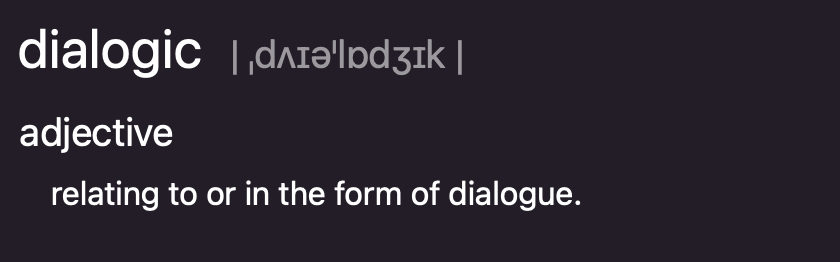
\includegraphics[width=6cm]{pictures/background/dialogic.png}
\caption{Dialogical engagement}{\autocite{Oxford_dictionary}}
\end{figure}


\subsection{Design as an interface for meaning making}
\autocite{kazmierczak_meaningmaking_2003} approaches design as an interface for meaning making, or simply the design of meaning. She see "meaning" as standing for a thought induced in the receiver, originated by contact with a design. According to her, design can be simple or complex in their material and conceptual structure but, as wholes, they are interfaces for meaning making \autocite[p. 47]{kazmierczak_meaningmaking_2003}. Borrowing from literature on cognitive semiotics, she proposes a model for design which relates physical form to cognition and comprehension rather than appearance and aesthetic. According to \autocite{kazmierczak_meaningmaking_2003}, there are two reasons why cognitive semiotics offers potentially good results; "First, it is focused on bridging the gap between form and meaning making or comprehension. Thus, its method of inquiry makes it well equipped for a discussion of symbolic-cognitive human phenomena such as communication. Second, it is compatible with the concerns of design regarding the construction of communications" \autocite[p. 47]{kazmierczak_meaningmaking_2003}. 
As I read it, Kazmierczak notions align with \autocite{Miekebal_book}'s writings on cultural analysis and discourses in the museum, the focus on cognitive semiotics as presented by Kazmierczak can prove useful and terms of better “reading”, describing and understanding a museum, exhibition or a specific installation through visiting a museum space. As we can see from the Oxford dictionary of English's definition of semiotic in Figure 2.6, it provides a concrete way of analysing the textual and written components, the signs and symbols, in a museum space. It enables the designer to see the museum agenda and curatorial function up against the designed object, and when working with interactivity to emphasise dialogic qualities it should be useful to have the means to see, discuss and question the semiotic aspects of the designed object. This way, the intersection between museal exposition, the museums exposition of arguments and their exposure of cultural and interactive artefacts can give the designer data or finds on power structures or tensions in the museum, in both analytical and evaluation stages of a design process.

\begin{figure}[H]
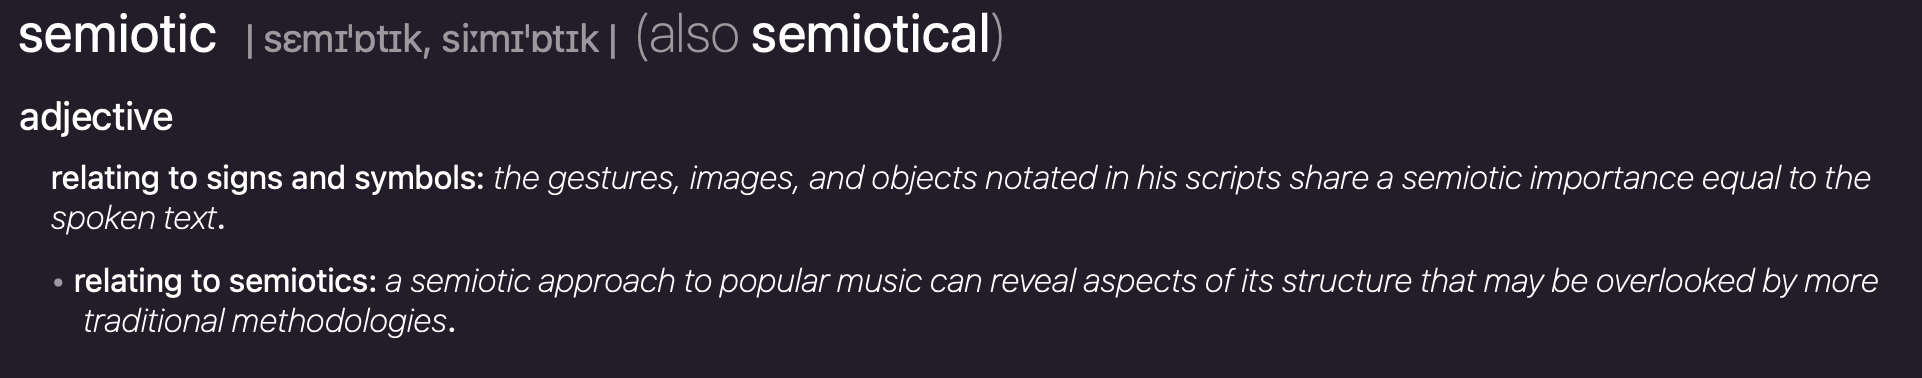
\includegraphics[width=12.5cm]{pictures/background/semiotic.png}
\caption{Semiotic perspective}{\autocite{Oxford_dictionary}}
\centering
\end{figure}


\section{Museology and the Anthropocene}
\emph{The Anthropocene} (Figure 2.7), refers to the present geological age, when humans are credited with having more impact on climate and planet than other factors combined \autocite{light_design_2017}, and is the museology term equal to the HCI community's notion on sustainability issues as a wicked problem. In a call for publication and participation to the conference "The future of tradition in museology" organized by ICOFOM in Kyoto 2019, the same institutional change and questions concerning the future of museology that we just have read through the eyes of \autocite{ross_interpreting_2015}, \autocite{vergo_museology_1989} and \autocite{vermeeren_museum_2018}, is addressed. They present five directions to be considered worthy of further research, whereas two of them stand out in term of this thesis's research interest. \autocite[p. 4]{icofom_kyoto_2019}:

\begin{itemize}
    \item \textbf{Museological tradition vs global development and new technologies:} What role does museology play and what position does it take in relation to the rapid changes that are taking place? (...), e.g. will cyberspace out rule other spaces and materialities – (...), considering the return to extreme political positions and the “war” of information and knowledge?
    \item \textbf{Museology and the Anthropocene:} How can museology reduce the disastrous effect man has on our planet earth and our living conditions? How can museology help to bridge the gap between mind and matter – the gap that is the reason for the state of mankind right now – the belief that man is superior to nature and all other creatures? (...) So what impact should this insight bring to our dealing with museums, objects and collections, with a sustainable future in mind?
\end{itemize}

\begin{figure}[H]
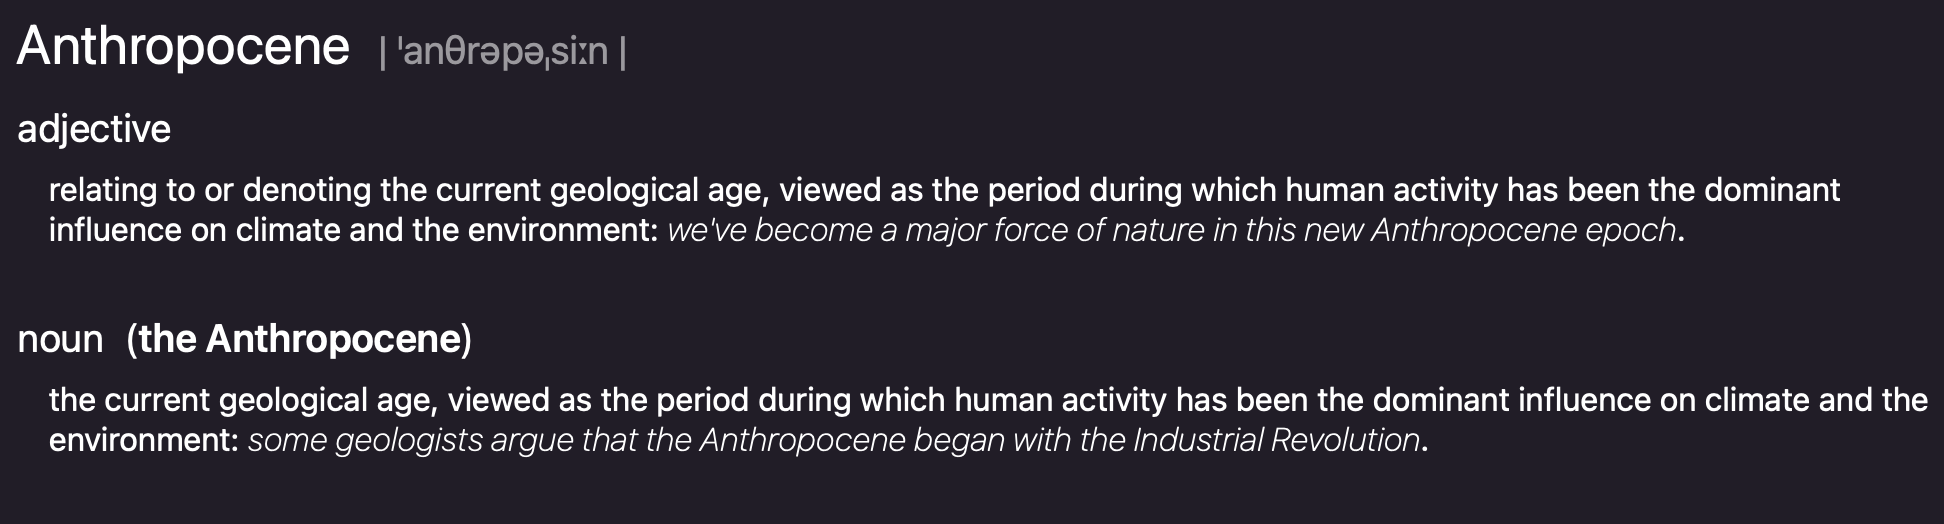
\includegraphics[width=12.5cm]{pictures/background/anthropocene.png}
\caption{The Anthropocene}{\autocite{Oxford_dictionary}}
\centering
\end{figure}

\subsection{Changing climate, changing attitude?}
"Many science museums and science centers now recognize their potential to arouse young peoples’ interest and awareness, and are starting to engage them in the climate change debate (e.g. Science Museum London, Australian Museum, Aquarium San Diego, American Museum of Natural History)" \autocite[p. 95]{gorr_changing_2014}. Studies show evidence of museum and science-centre experiences resulting in attitude change \autocite{smithsonian_2011}, and evidence from a range of environmental-related exhibitions that initial changes in attitude and understanding fade after a couple of weeks because museum visitors tend to seek confirmation of their pre-existing attitudes and cling to erroneous beliefs \autocite{Cakir_2008}. "Some examples have even illustrated that attempts to increase people’s understanding of climate change enhanced skepticism and resulted in visitors’ total rejection of the issue \autocite{guardian_2009}". "Aiming to examine attitude changes in young people, the described study drew on general findings about attitude from social sciences and psychology \autocite[p. 96]{gorr_changing_2014}. "A closer look at the theory reveals that attitude is a highly complex and ambivalent term; for instance, a person may want to express both positive and negative attitudes toward the same object" \autocite[p. 96]{gorr_changing_2014}. "Whether an experience leads to longer lasting attitude change depends on numerous aspects such as motivation and attention" \autocite[p. 96]{gorr_changing_2014}. "Motivation is mostly dependent on clarity and on the personal relevance of a message [\autocite{salazar_mediations_2011}], or it may result from emotions, such as empathy and enjoyment [\autocite{Roberts_1997}]" \autocite[p. 96]{gorr_changing_2014}.

\break
\subsection{The museum as change agent}
A commentary by Richard J. Hebda looks into the Royal British Columbia Museum (RBCM)’s voyage into the issue of climate change as an example of how museums can play a central role in addressing contemporary issues. Traditionally, museums have been a window to the past, \emph{a place where the past lives} \autocite[p. 1]{hebda_article}. Many of the issues and societal attitudes addressed in the commentary are still relevant today; traditionally, human and natural history have been seen as two museum fictions, solitudes, that have been exhibited separately. A key appeal for the RBCM, (a typical natural history museum) to do a climate change exhibit, was to pursue the opportunity to link and integrate the two solitudes in a compelling and relevant manner \autocite[p. 2]{hebda_article}. They justify that the combining of the two is necessary because in the sustainability debate, the separation of the two is at the core of the problem facing society today \autocite[p.2]{hebda_article}. In 2007 when the RBCM decided to make the climate change exhibition, the question of climate change was still a controversial issue \autocite[p.2]{hebda_article}. Addressing the increasing evidence and knowledge in terms of climate change and how it affects and is affected by humans, nearly all reputable scientists felt that change was underway, and action was needed \autocite[p.2]{hebda_article}. However, the political and public atmosphere was foggy, as people did not know whom to believe, what information was science-based rather than rhetoric, and where real uncertainty lay \autocite[p.2]{hebda_article}. The RBCM saw a clear opportunity to dispel the fog and to enlighten their audiences \autocite[p.2]{hebda_article}.

"One of the key terms today is learning in formal and informal contexts. Museums, too, are redefining their mission; instead of focusing on collecting and classifying, the emphasis is now on exhibition design and the museum as a place for communication and learning" \autocite[p. 8]{insulander_designs_2009}. "Social research underlines how the mass media frames and presents environmental change and risk in ways that become contested cultural constructs embedded in deep ideological structures" \autocite[p. 1]{salazar_mediations_2011}." While significant attention has concentrated on the mass media, less consideration has been given to examining the role of museums and science centers in communicating the science of climate change" \autocite[p. 1]{salazar_mediations_2011}. In the article \emph{The mediations of climate change: museums as citizens media}, Salazar looks at museums as being cultural brokers around the public understanding of climate change. By engaging with recent conceptualizations around citizens and public media practices, Salazar proposes mechanisms through which the museum sector can act as change agents in fostering a new form of public pedagogy that incorporates differing civic epistemologies around climate change education and action" \autocite[p. 1]{salazar_mediations_2011}.


Salazar and Hebda highlight how the museum sector is beginning to act as change agents, specifically in climate change education and action. Surveys from, for example, the USA show that museums score higher on trust than other institutions, such as media and government agencies, and that the credibility of museums continues to increase during the pandemic \autocite{impact_2020}. As important actors in the public discourse, it is crucial for museums in the future that they defend this position and further develop it. It is essential to secure a position where a room is created for different opinions to meet and break and counter the emergence of echo chambers, conspiracy theories, and false news \autocite[p. 41]{melding23}.